\documentclass[12pt]{article}
\usepackage[utf8]{inputenc}
\usepackage{amsmath}
\usepackage{hyperref}
\usepackage{graphicx}
\usepackage[swedish]{babel}
\title{Andragradsfunktioner}
\date{}
\begin{document}
  \maketitle
  
  
  
  \section{Introduktion}
  Det här dokumentet kommer från en fritt tillgänglig text på webbplatsen GitHub (se \url{https://github.com/Itangalo/Andragradsfunktioner}).
  Alla som är intresserade är inbjudna att föreslå och diskutera ändringar och förbättringar.
  Det kan man antingen göra genom att starta diskussioner i projektets ``issue queue'' (alternativt kommentera i befintliga diskussioner), eller genom att göra en kopia (``klon'') av hela projektet och redigera så mycket man vill.
  Om man är nöjd med sina ändringar, och vill att de ska tas in i ursprungliga dokumentet, kan man markera detta -- så kan förslaget diskuteras av andra inblandade.

  Innehållet i det här projektet är tillgänglig under Creative Commons-licens \href{http://creativecommons.org/licenses/by-nc-sa/3.0/}{attribution+non-commercial+share alike}.


  \section{Första skisser}
  
  (Det här är bara första skisser på upplägg av innehåll i dokumentet.)

  \subsection{Översikt av egenskaper för andragradsfunktioner.}
  Andragradsfunktioner har en högsta eller lägsta punkt, vilket gör dem användbara för att modellera vissa typer av samband.
  (Utgångspunkt i sådana samband!)
  Vad extrempunkt och extremvärde betyder, och varför de är viktiga begrepp i tillämpad matematik.

  \subsection{Hur uttrycket $f(x) = a(x+d)^2+e$ beter sig}
  Det finns olika sätt att representera andragradsuttryck, och $a(x+d)^2+e$ är en form som är praktisk för att se engenskaper hos funktioner.
  Utforskande av hur de olika parametrarna påverkar funktionens graf, framförallt hur $d$ och $e$ hänger samman med extrempunkt/extremvärde.
  (Bifogad GeoGebra-demonstration!)
  Fördjupning: Parametrarna $d$ och $e$, och translation av funktioner.
  
  \subsection{Andragradsekvationer}
  Motivering av ekvationer av typen $a(x+d)^2+e=k$.
  Hur man löser sådana ekvationer, med utgångspunkt i potensekvationen $x^2 = k$.
  Fördjupning: Jämförelse med substitutionen $t=x+d$.

  \subsection{Kvadratkomplettering med ansättning}
  Introduktion av andragradsuttryck på formen $ax^2+bx+c$, och hur parametern $c$ avspeglas i funktionens graf.
  Resonemang kring att det finns något uttryck $a(x+d)^2+e$ som representerar varje uttryck på formen $ax^2+bx+c$.
  Kvadreringsregler: utveckla uttryck på formen $(a+b)^2$ eller $(a-b)^2$.
  (Inklusive länk till digital mängdträning, som även omfattar andra parentesmultiplikationer.)
  Hur man kan översätta formen $ax^2+bx+c$ till kvadratkompletterad form (genom ansättning).
  Fördjupning: Vad ansättning egentligen innebär.
  
  \subsection{Överblivet}
  \begin{itemize}
    \item Faktorisering som genväg för att lösa andragradsekvationer
    \item Konjugatregeln. (Ha tillsammans med kvadreringsreglerna?)
    \item Komplexa tal och komplexa lösningar till andragradsekvationer
    \item Hur man kan hitta parametrarna $a$/$d$/$e$ eller $a$/$b$/$c$ från givna punkter
    \item Symmetrilinje för andragradsfunktioner
  \end{itemize}
  
  \begin{figure}
  \centering
  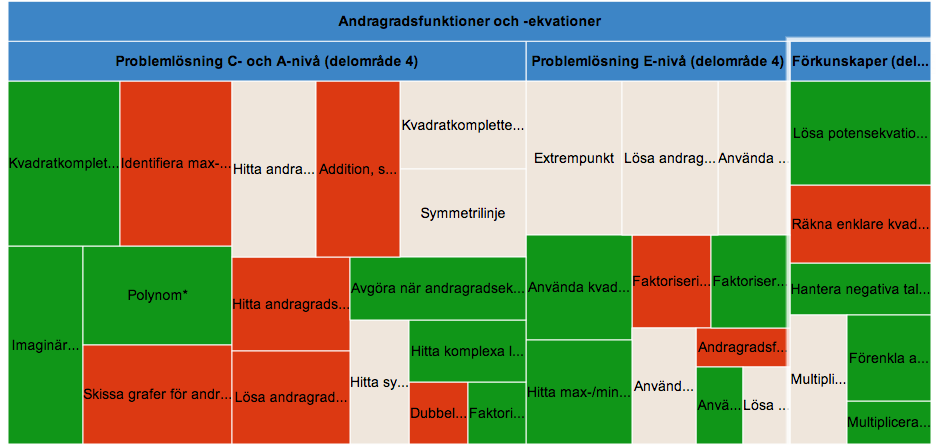
\includegraphics[width=0.3\textwidth]{bilder/testbild.png}
  \caption{\label{fig:testbild}Det här är bara ett test, för att se hur det fungerar att bädda in bilder.}
  \end{figure}


\end{document}
